\documentclass[a4paper]{article}
\usepackage[utf8]{inputenc}
\usepackage{polski}
\usepackage{graphicx}

%\usepackage{geometry}
%\newgeometry{tmargin=2.5cm, bmargin=2cm, lmargin=2cm, rmargin=2cm}

\title{Pół-autonomiczny pojazd czterokołowy}
\author{Jędrzej Maliniak \and Piotr Hebel \and Filip Malinowski \and Piotr Dulewicz \and Piotr Jabłoński \and Andrzej Szmyt}
\date{7 marca 2016}

\begin{document}

\maketitle

\section{Problem projektu}
    Przedmiotem tego projektu jest pół-autonomiczny pojazd czterokołowy wyposażony w kamerę, sensory mierzące odległość wykorzystywane do orientacji, zbierania danych, a także do unikania zderzeń z przeszkodami niezależnych od woli sterującego (opóźnienia w transferze danych z kamery). W przyszłości zespół ma nadzieję na rozwój projektu wzbogacając go o m.in. możliwość mapowania otoczenia, umożliwić interfejs do komunikacji z montowanym działem laserowym czy prostym manipulatorem/ramieniem/chwytakiem umożliwiającym zbieranie próbek terenu czy wykonywanie prostych operacji na napotkanych obiektach.
    
    Spodziewany wynik prac to wyżej opisany zdalnie sterowany pojazd bezzałogowy umożliwiający np. zbieranie informacji na temat nowych miejsc o nieznanych warunkach środowiskowych, pobieranie próbek z miejsc objętych skażeniem, czy wykorzystanie w wojsku. Jest to ważny temat umożliwiający człowiekowi interakcję w miejscach, warunkach, w których ta interakcja byłaby niewskazana czy wręcz niebezpieczna. 

    Wyniki będą umieszczane w archiwum z oprogramowaniem wraz z dokumentacją algorytmów, oprogramowania, układu mechanicznego i elektronicznego oraz przykładami działania.
\section{Plan pracy}
    Na następnej stronie znajduje się wykres Gantta prezentujący podział oraz rozplanowanie zadań w czasie.
    
        \begin{figure}
            \centering
            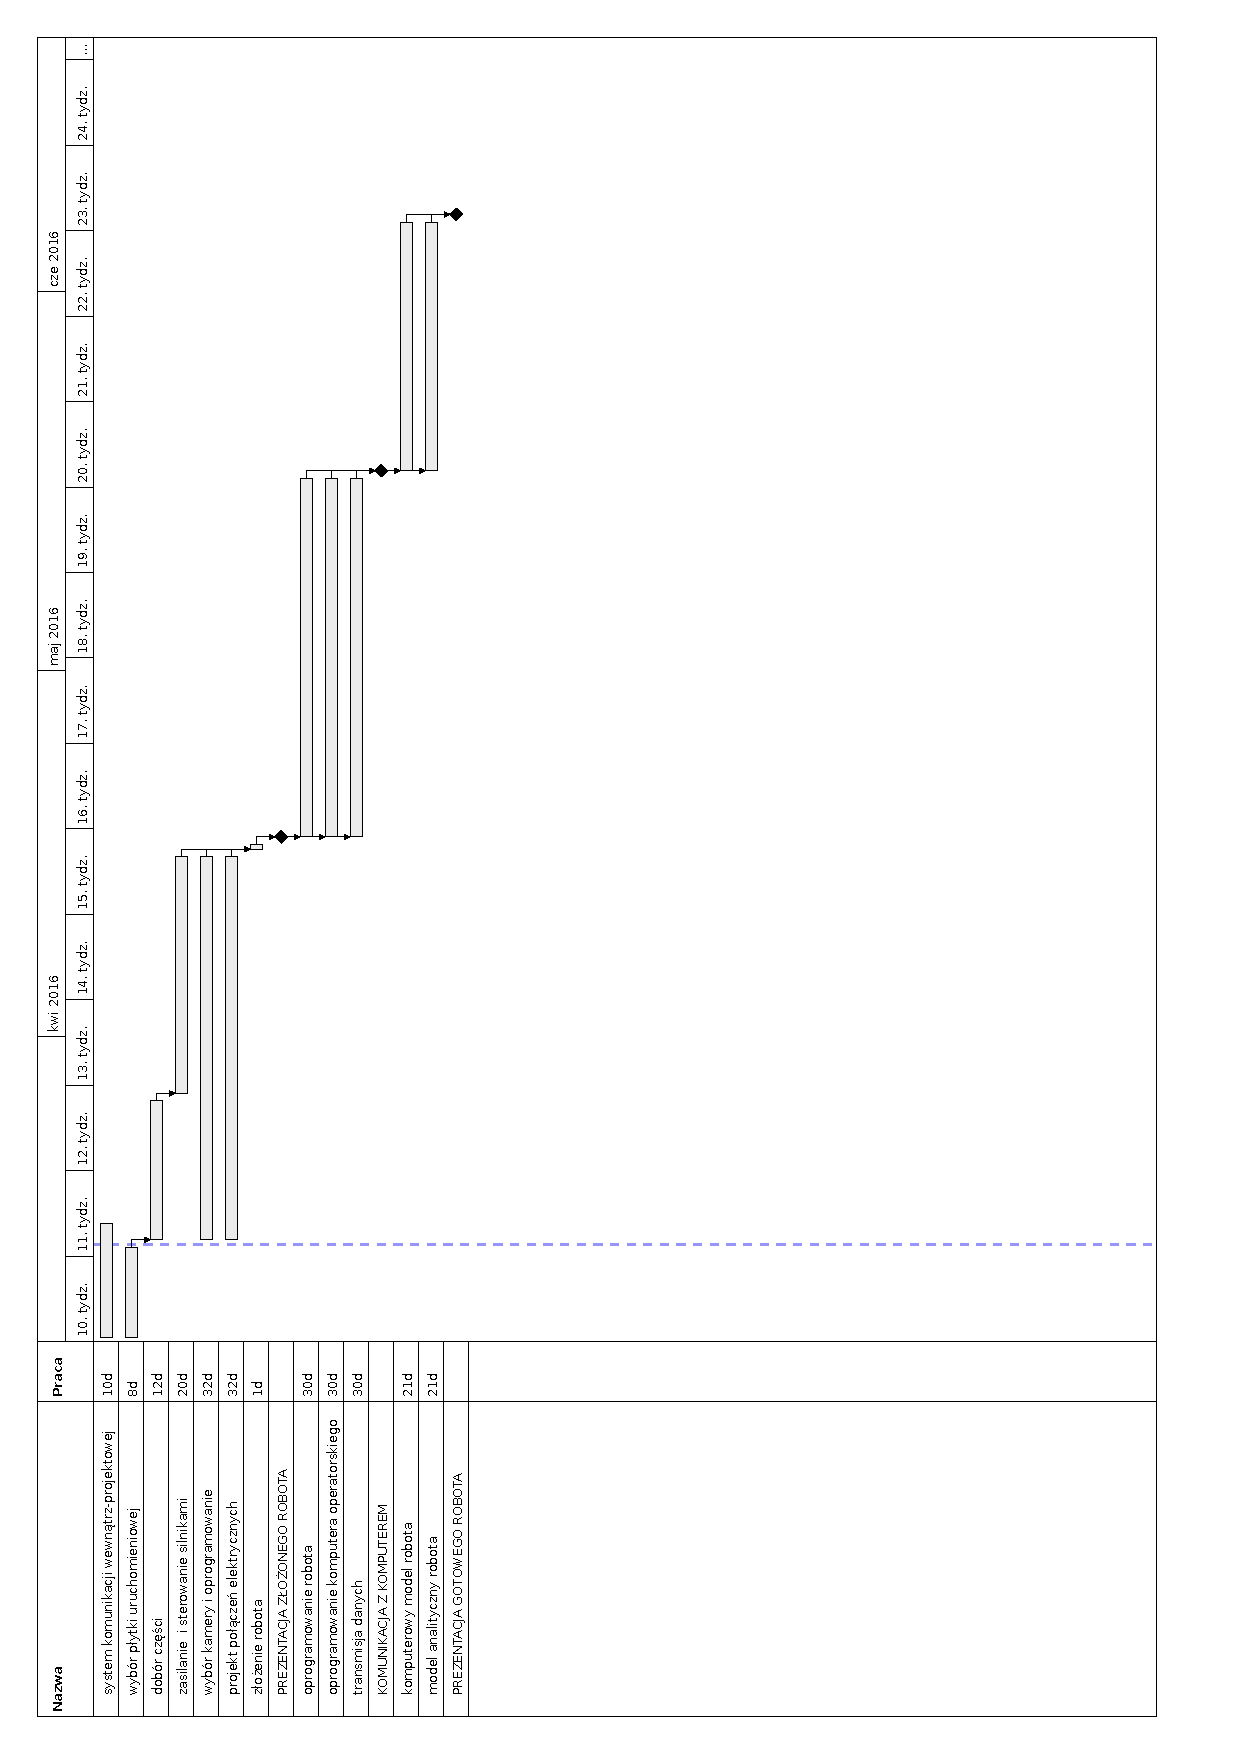
\includegraphics[scale=0.7]{gantt}
            \label{fig:my_label}
        \end{figure}
        
\section{Doręczenie}
    Raporty i postępy będą prezentowane w terminach zaznaczonych w diagramie Gantta jako kamienie milowe.
\section{Budżet}
    Sekcja budżetu jest opcjonalna i wymaga uzupełnienia.
\section{Zarządzanie projektem}
    \subsection{Standardy wykorzystywane podczas pracy nad projektem}
    \begin{itemize}
        \item \LaTeX - do tworzenia dokumentacji
        \item planner - do tworzenia diagramu Gantta
        \item git - zdecentralizowany system do kontroli wersji
        \item trac - do rozdzielania zadań do wykonania (współpracuje z gitem)
        \item doxygen - do dokumentowania kodu
        \item TopSolid - do tworzenia komputerowego modelu robota
    \end{itemize}
    Regularne spotkania będą odbywały się w uprzednio wybrany dzień weekendu. Konflikty będą poddawane demokratycznej debacie a w razie braku konsensusu koordynator ma rozstrzygający głos.
\section{Zespół}
    \subsection{Jędrzej Maliniak}
    Koordynator projektu - przydzielanie i nadzór zadań wykonywanych przez członków grupy, zarządzanie projektem.
        \begin{itemize}
            \item Budowa robota
            \item Oprogramowanie robota
            \item Kwestia komunikacji bezprzewodowej
            \item Opracowanie algorytmów
            \item Kwestie programistyczne
        \end{itemize}
    \subsection{Piotr Dulewicz}
        \begin{itemize}
            \item Oprogramowanie robota
            \item Projekt komputerowy
        \end{itemize}
    \subsection{Piotr Hebel}
        \begin{itemize}
            \item Budowa robota
            \item Kwestia komunikacji bezprzewodowej
            \item Projekt komputerowy
        \end{itemize}
    \subsection{Filip Malinowski}
        \begin{itemize}
            \item Opis analityczny
            \item Opracowanie algorytmów
            \item Kwestie programistyczne
            \item Projekt komputerowy
        \end{itemize}
    \subsection{Piotr Jabłoński}
        \begin{itemize}
            \item Budowa robota
            \item Kwestie programistyczne
            \item Projekt komputerowy
        \end{itemize}
    \subsection{Andrzej Szmyt}
        \begin{itemize}
            \item Budowa robota
            \item Kwestia komunikacji bezprzewodowej
            \item Projekt komputerowy
        \end{itemize}
        

\end{document}

